%\documentclass[tikz, border=5pt]{standalone}
\begin{document}
	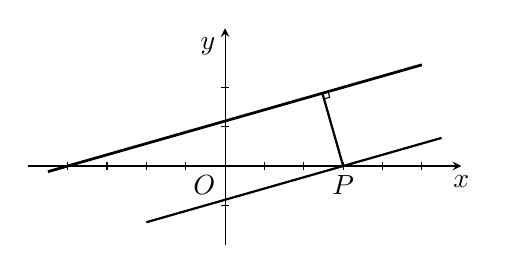
\begin{tikzpicture}[>=stealth, scale=0.5] % 箭头样式为stealth,
		
		% 绘制坐标轴
		\draw[->] (-5,0) -- (6,0) node[below] {$x$}; % x轴(带箭头和标签)
		\draw[->] (0,-2) -- (0,3.5) node[below left] {$y$}; % y轴(带箭头和标签)
		\node at (0,0) [below left] {$O$};           % 原点O的标签
		
		% 绘制所有小刻度线(从 -1 到 2,每隔 1 单位画竖线)
		\foreach \x in {-4,-3,...,5} {
			\draw (\x, 0.1) -- (\x, -0.1);  % 小竖线(长 0.2 单位)
		}
		\foreach \y in {-1,0,...,2} {
			\draw (0.1,\y) -- (-0.1,\y);  % 小竖线(长 0.2 单位)
		}
		
		% 绘制直线l 7y=2x+8
		\draw[line width=1pt] (-4.5,-1/7) -- (5,18/7) ;
		% 绘制直线l 7y=2x-6
		\draw[thick] (-2,-10/7) -- (5.5,5/7) ;
		
		% 交点: (131/53, 98/53)
		\draw[thick] (3, 0) -- ++({180-atan(3.5)}:1.95);
		% 直角符号
		\draw (131/53, 98/53) -- ++({atan(2/7)}:0.15) -- ++({atan(2/7)-90}:0.15) -- ++({atan(2/7)-180}:0.15);
%		\draw (2.47, 1.85) -- ++({atan(2/7)}:0.15) -- ++({atan(2/7)-90}:0.15) -- ++({atan(2/7)-180}:0.15);
		
		% 标记各点的标签
		\node at (3,0) [below] {$P$};
		
	\end{tikzpicture}
\end{document}
